% Last Modified: Fri Sep 09, 2011 at 15:17

\documentclass{article}
\usepackage{cite, listing, graphicx, subfigure, amsmath}
% correct bad hyphenation here
\hyphenation{fault-tolerant fault-tolerance hash-table bit-Torrent}

\begin{document}

\title{Topology Management in Peer-to-Peer Systems}
\author{Jorge J.~G\'omez}

\maketitle
\section{Problem Statement}
  Using an algorithm based on the paper~\cite{t-man} by Jelasity and
  Babaoglu, this assignment asked to simulate a distributed node system
  managing it's topology. The algorithm involves having the nodes
  trading neighbor lists and selecting the closest nodes based on two
  distinct distance formulas. The result is that after a certain amount
  of cycles, the topology begins to converge to the optimal.
\section{Approach}
  Following the notes in the assignment, the algorithm was created in
  Python 2.7.1. The nodes where instantiated as objects that had a
  gossip method in which the node would trade neighbor lists with one of
  its neighbors. The node would then select the $k$ closest nodes, where
  $k$ is an input parameter. The node class had other methods for
  finding the distance to a given node and choosing the closest
  neighbors.  The distance formula changes depending on the command line
  input with either a 1 dimensional distance or 2 dimensional Eucledian
  distance (chord distance on a unit circle).  Another class was made to
  help set up a system and simulate it.  More information can be found
  in the source code
  \texttt{hw1.py}.
\section{Results and Figures}
  The code was written with unit tests to ensure every step of
  development was correct and development proceeded without major
  issues.  Figure~\ref{results1} shows the plot for a one-dimensional
  distance simulation. The system converges to a total distance of
  120,000. Figure~\ref{results2} shows the plot for a two-dimensional
  distance simulation. The system converges to a total distance of 505.

  \begin{figure}[h]
    \centering
    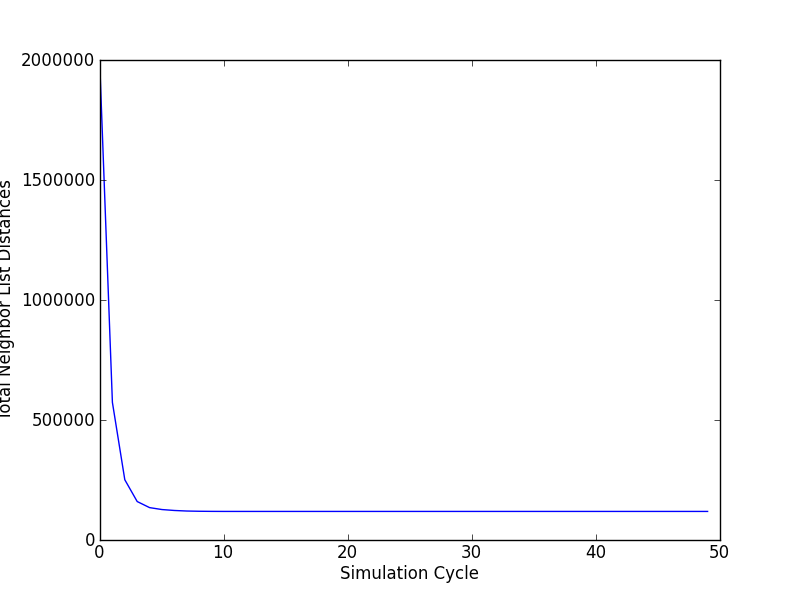
\includegraphics[width=1\textwidth]{simData1D.png}
    \caption{Total Distances in Neighbors over 50 simulation cycles with system
    size of 1000 nodes, neighbor list length of 20, and 1-D distances.}
    \label{results1}
  \end{figure}

  \begin{figure}[h]
    \centering
    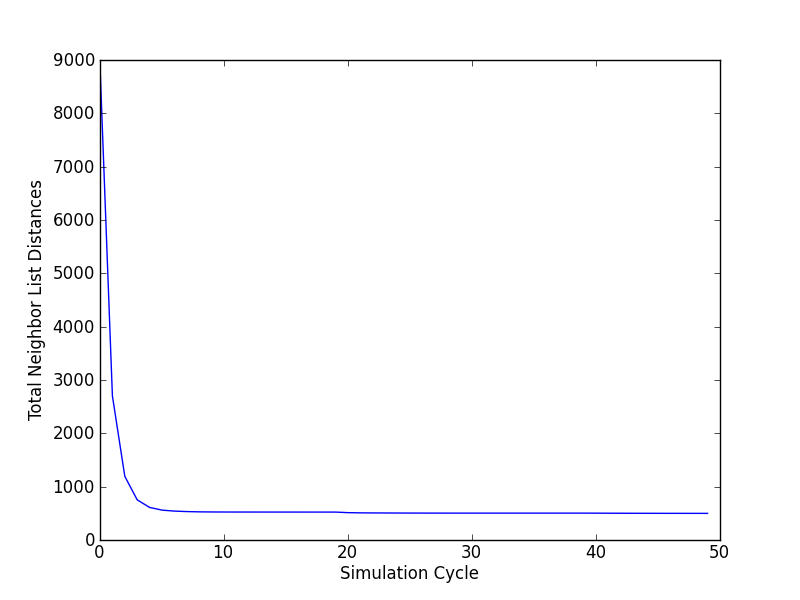
\includegraphics[width=1\textwidth]{simData2D.png}
    \caption{Total Distances in Neighbors over 50 simulation cycles with system
    size of 1000 nodes, neighbor list length of 20, and 2-D distances.}
    \label{results2}
  \end{figure}

\newpage
\bibliographystyle{plain}
\bibliography{dist.bib}

\end{document}
